\documentclass[./\jobname.tex]{subfiles}
\begin{document}
%
% A textual specification of the requirements of the system.
% A use-case diagram of the system.
% A sequence diagram of one scenario.
% An activity diagram of one scenario.
% The scenario used for the latter two diagrams can be the same.
%
\chapter{Anforderungen}
%
In diesem Kapitel wird die allgemeine Funktion mithilfe von Use-Case Diagrammen, Sequenz Diagrammen und Activity Diagrammen beschrieben. Anschließend werden die \gls{fr} und \gls{nfr} in Tabellenform kurz und prägnant dargestellt.
%
\section{Use-Case Diagramm}
%
In \autoref{fig: Use-case-diagram.pdf} ist der Use-Case für das \gls{cb} dargestellt. Es gibt im gesamten vier Akteure:
%
\begin{description}
	\item[User] Dieser Akteur ist für den Service-Betriebsmodus vorgesehen und führt an einem Förderband Operationen im \modeA durch. Der User erhält volle Kontrolle über alle möglichen Funktionen des Förderbandes. Durchgeführt wird die Kommunikation entweder über die lokale Tastatur oder über eine \gls{telnet}-Verbindung.
	\item[Master] Dieser Akteur ist nur im \modeB vorhanden. Er vermittelt den Förderbändern die jeweils rechten Nachbarn und übergibt einem der Förderbänder in der Kette ein Paket und initiiert somit den Start der Förderbänder. Diese Kommunikation erfolgt über Standard Ethernet.
	\item[left \gls{cb}] Dieser Akteur ist nur im \modeB vorhanden. Er dient dazu, die Kommunikationsanforderungen zwischen dem linken und dem eignen Förderband darzustellen. Diese Kommunikation erfolgt über Standard Ethernet.
	\item[right \gls{cb}] Dieser Akteur ist nur im \modeB vorhanden. Er dient dazu, die Kommunikationsanforderungen zwischen dem eigenen und dem rechten Förderband darzustellen. Diese Kommunikation erfolgt über Standard Ethernet.
\end{description}
%
Es gibt im gesamten 4 Use-Cases die die Funktionalität des zu entwerfenden Systems beschreiben:
%
\begin{description}
	\item[Operating Mode] Hier erfolgt die Auswahl zwischen \modeA und \modeB
	\item[Local Mode] Betrieb im \modeA
	\item[Chain Mode / Packet transport] Betrieb im \modeB
	%\item[Communication] Dient der Nachrichtenübermittelung zum Förderband über \gls{telnet}, \gls{tcp}/\gls{ip} oder über das Tastaturfeld.
	\item[Set right \gls{cb} \acrshort{ip}] Dient zur Initialisierung der Förderkette und weist die jeweiligen rechten Nachbarn zu.
\end{description}
%
\begin{figure}[H]
	\centering
	\noindent\adjustbox{max width=\textwidth}{%falls größer als \textwidth, wird das Bild verkleinert
		%trim option's parameter order: left bottom right top
		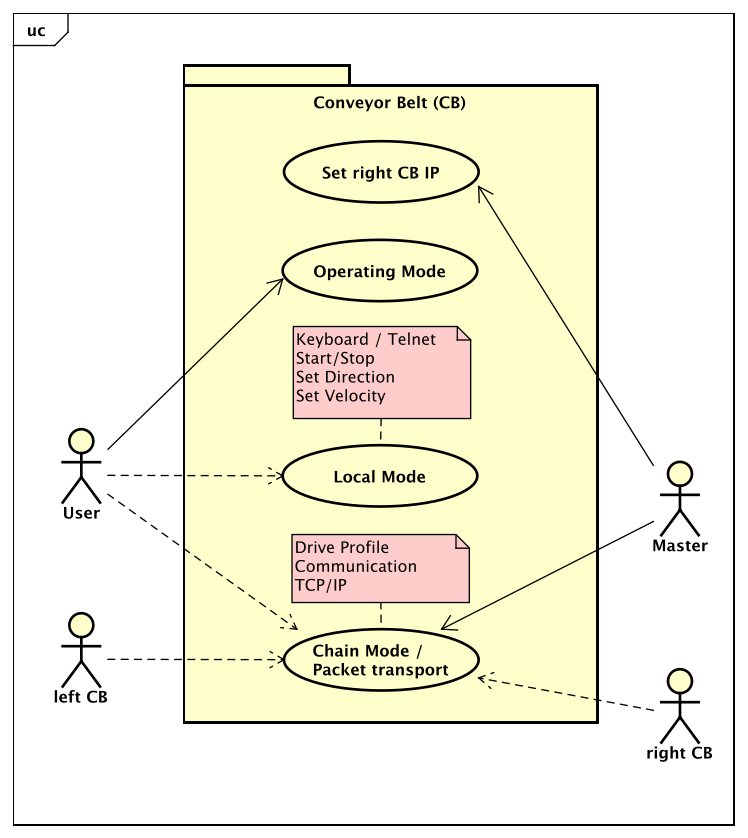
\includegraphics[width=1\textwidth]{./img/1_Anforderungen/Use-case-diagram.pdf}
	}
	\unterschrift{Use-Case Diagramm}{eigene Ausarbeitung}{}
	\label{fig: Use-case-diagram.pdf}
\end{figure}
%
\section{Sequenz Diagramm}
%
In \autoref{fig: initialization_of_the_chain.pdf} ist das Sequenzdiagramm dargestellt. Es zeigt die Initialisierung der Förderbandkette durch den Master.
Dieser übergibt nach der Vermittlung der jeweiligen rechten Nachbarn das zu transportierende Paket eines Förderbandes, die daraufhin den Ablauf zum Fördern starten. Als Master im \modeB ist ein beliebiger Rechner der FHV gedacht.
%
\begin{figure}[H]
	\centering
	\noindent\adjustbox{max width=\textwidth}{%falls größer als \textwidth, wird das Bild verkleinert
		%trim option's parameter order: left bottom right top
		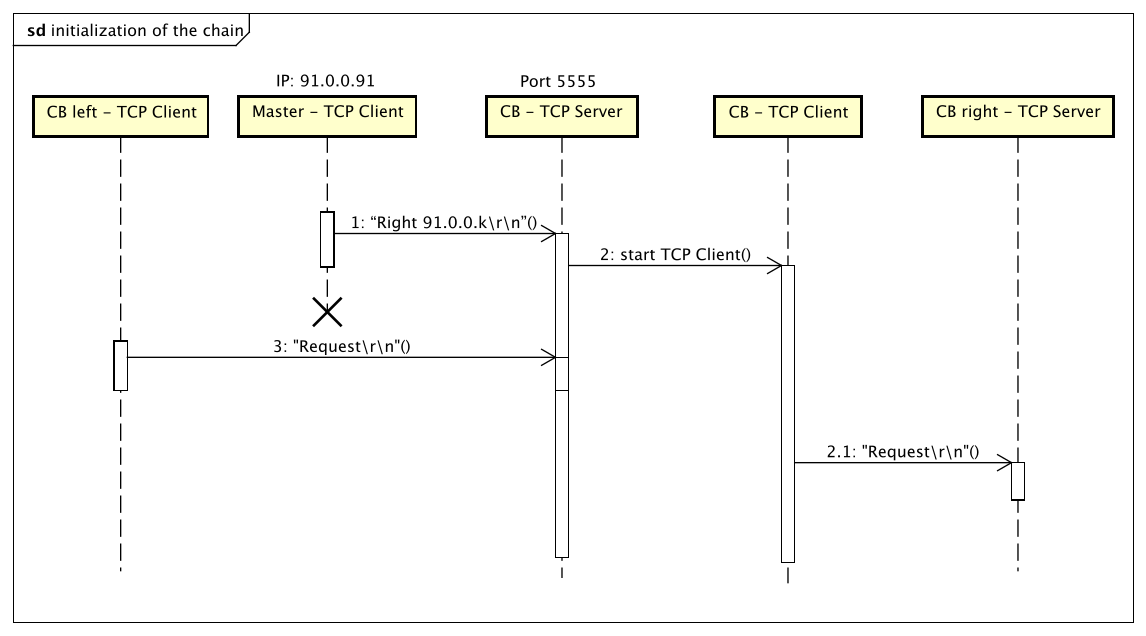
\includegraphics[width=1\textwidth]{./img/1_Anforderungen/initialization-of-the-chain.pdf}
	}
	\unterschrift{Initialisierung}{eigene Ausarbeitung}{}
	\label{fig: initialization_of_the_chain.pdf}
\end{figure}
%
\section{Activity Diagramm}
%
In \autoref{fig: Activitaetsdiagramm_Programmauswahl} ist das Aktivitätsdiagramm dargestellt. Es beschreibt den \modeA und \modeB.\par
%
Im \modeB muss das virtuelle Förderband nur \paket{e} von links nach rechts befördern. Es soll gewartet werden, bis von links eine Anfrage gesendet wird, dass ein \paket{} vorhanden ist. Wird gerade eine Bewegung ausgeführt, so muss mit \wait geantwortet werden. Andernfalls wird mit \ready geantwortet und für eine Zeitdauer von \timeTpp mit einer langsamen Geschwindigkeit von \(100~U/min\) in Richtung zum rechten Förderband gefahren. Nach Ablauf der Zeitdauer \tpp wird das linke Förderband mit \release informiert, dass das Paket erfolgreich übernommen wurde. Ebenfalls wird jetzt das definierte Geschwindigkeitsprofil aktiviert.\par
Ist das Geschwindigkeitsprofil beendet, wird eine \request Anfrage zum rechten Förderband gesendet, um festzustellen, ob dieses bereit ist. Wird die Anfrage mit \wait quittiert, so wird das Förderband gestoppt. Jedoch bei Quittierung mit \ready, wird die Geschwindigkeit auf \(100~U/min\) reduziert, bis \release empfangen wurde. Jetzt kehrt das Förderband wieder in den Ruhezustand zurück und stoppt den Motor.\par
%
Der \modeA unterscheidet sich im wesentlichen zum \modeB, dass die Förderbänder autark arbeiten. Der \modeA ist somit unabhängig und kein Teil der Förderkette und dadurch entfällt jegliche Kommunikation zur Außenwelt, bis auf die \gls{telnet}-Verbindung zur Steuerung.\par
%
In \modeA kann zuerst die Richtung der Förderbewegung und die Drehzahl im Bereich von \minMaxVelocity in Schritten von \stepSizeMotor eingestellt werden. Die Benutzerinteraktion erfolgt durch das Keyboard und Display oder \gls{telnet}.
%Der Local Mode ist ebenfalls an jeder Stelle durch Betätigen der Stoptaste unterbrechbar.
%
\begin{figure}[H]
	\centering
	\noindent\adjustbox{max width=\textwidth}{%falls größer als \textwidth, wird das Bild verkleinert
		%trim option's parameter order: left bottom right top
		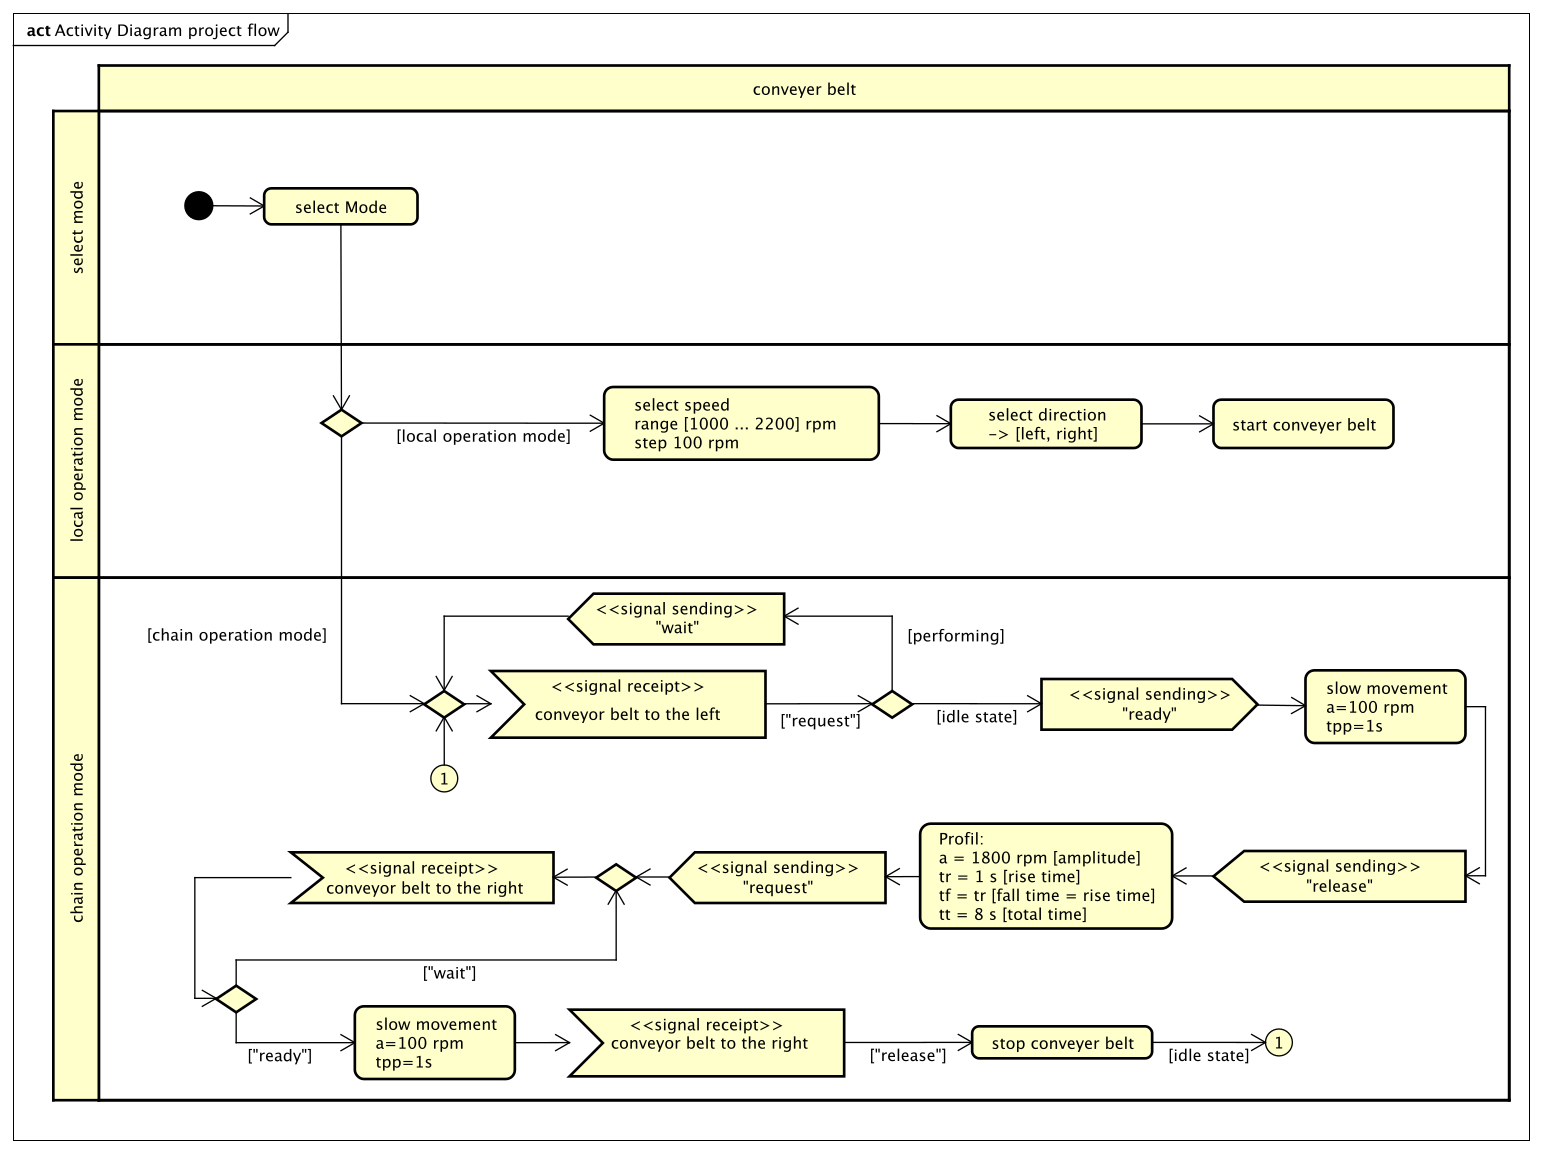
\includegraphics[width=1\textwidth]{./img/1_Anforderungen/Activitaetsdiagramm_Programmauswahl}
	}
	\unterschrift{Aktivitätsdiagramm}{eigene Ausarbeitung}{}
	\label{fig: Activitaetsdiagramm_Programmauswahl}
\end{figure}
%
\section{Funktionale und nicht Anforderungen}
%
Die funktionalen Anforderungen wurden zur besseren Übersicht in drei Teile gegliedert:
%
\begin{itemize}
	\item Allgemeine funktionale Anforderungen
	\item Funktionale Anforderungen für \modeA
	\item Funktionale Anforderungen für \modeB
\end{itemize}
%
\begin{table}[H]
	\centering
	\noindent\adjustbox{max width=\textwidth}{%falls größer als \textwidth, wird das Bild verkleinert
		\begin{threeparttable}
			\begin{tabular}{Y{0.5cm}Y{0.75cm}Y{2.65cm}m{10cm}}
				\toprule
				\textbf{Nr.} & \textbf{\acrshort{fr}\tnote{a} \acrshort{nfr}}\tnote{b}    & \textbf{Verbindlichkeit}  & \textbf{Beschreibung}  \\ \toprule
				\getReqCtr{req:1} & \acrshort{fr} & muss & Das Förderband muss zwei Betriebsmodi unterstützen. Den \modeA und \modeB. 	\\ \hline
				%\getReqCtr{req:2} & \acrshort{fr} & muss & Das Förderband muss fähig sein, eine Palette von der linken Seite zur rechten Seite zu transportieren.	\\ \hline
				\getReqCtr{req:3} & \acrshort{fr} & muss & Das System muss hingehend erweiterbar sein, sodass Förderbänder beliebig hinzugefügt bzw. entfernt werden können.	\\ \hline
				\getReqCtr{req:4} & \acrshort{fr} & muss & Das Förderband muss einen \acrshort{ptp}-Client implementiert haben, um die Uhrzeit zum Master zu synchronisieren. Der Code wird vom Auftraggeber zur Verfügung gestellt. \\ \hline
				\getReqCtr{req:5} & \acrshort{nfr} & muss & Das \acrshort{ptp} muss  Port 5432 verwenden. \\ \hline
				\getReqCtr{req:6} & \acrshort{fr} & muss & Die Geschwindigkeit muss über eine geschlossene Reglerschleife geregelt sein. Der benötigte Code wird vom Auftraggeber zur Verfügung gestellt.  \\ \hline
				%\getReqCtr{req:7} & \acrshort{fr} & muss & Das Display muss die notwendigen Informationen anzeigen. \\ \hline
				\getReqCtr{req:8} & \acrshort{fr}& soll & Die in \cite{pilsan2014} definierten Funktionen sollten für den Zugriff der Hardware verwendet werden. In diesem Dokument werden die notwendigen Funktionen für den Zugriff der Hardware beschrieben. \\ \hline
				\getReqCtr{req:9} & \acrshort{fr} & muss& Das Keyboard muss als Eingabe fungieren. Die Tastenbelegung ist unter \autoref{fig: funktionen tastenfeld} ersichtlich. \\ \hline
				\getReqCtr{req:10} & \acrshort{fr} & muss& \gls{telnet} muss als Eingabe fungieren. Die Telegramme sind unter \autoref{tab: telnet kommunikation} ersichtlich. \\ \hline
				\getReqCtr{req:11} & \acrshort{nfr}& muss & Der \gls{telnet}-Server muss den Port 4444 verwenden. \\ \hline
				\getReqCtr{req:12} & \acrshort{nfr} & muss& \(a\) und \(\omega\) müssen \(\pm 50~U/min\) genau erreicht werden.\\ \hline %\(a, \omega \pm 50 rpm\)
				\getReqCtr{req:13} & \acrshort{nfr} & muss & Das Förderband muss folgende Informationen am Display ausgeben (siehe \autoref{fig: display})
				\begin{itemize}
					\item Angewählter Betriebsmodus
				\end{itemize}\\ \hline
			\getReqCtr{req:14} & \acrshort{nfr} & soll & Die \acrshort{ptp} Implementierung kann vom Auftraggeber übernommen werden. \\ \hline
			\getReqCtr{req:14} & \acrshort{nfr} & muss & Die \acrshort{ptp} Updaterate (\enquote{Sync} Message) ist auf \(4\) Sekunden gestellt und verwendet nicht Multicast. \\ \hline
			\getReqCtr{req:14} & \acrshort{nfr} & muss & Das Feld \enquote{Nanoseconds} des \glsentryshort{ptp} ist immer null. \\ \hline	
			\end{tabular}
			
			\unterschrift{Allgemeine funktionale Anforderungen}{eigene Ausarbeitung}{}
			\label{tab: Allgemeine funktionale Anforderungen}
			\begin{tablenotes}
				\footnotesize
				\item [a] \acrfull{fr}
				\item [b] \acrfull{nfr} 
			\end{tablenotes}
		\end{threeparttable}
	}
\end{table}
%
%\begin{table}[H]
%	\centering
%	\noindent\adjustbox{max width=\textwidth}{%falls größer als \textwidth, wird das Bild verkleinert
%	\begin{threeparttable}
%	\begin{tabular}{Y{0.5cm}Y{0.75cm}Y{3.45cm}Y{2.65cm}m{7.5cm}}
%		\toprule
%		\textbf{Nr.} & \textbf{\acrshort{fr}\tnote{a} \acrshort{nfr}}\tnote{b}    & \textbf{Teil}            & \textbf{Verbindlichkeit}  & \textbf{Beschreibung}  \\ \toprule
%		\getReqCtr{} & \acrshort{fr}  & Das Förderband & muss & zwei Betriebsmodi unterstützen. Den \modeA und \modeB. 	\\ \hline
%		\getReqCtr{} & \acrshort{fr}  & Das Förderband & muss & fähig sein, eine Palette von der linken Seite zur rechten Seite zu transportieren.	\\ \hline
%		\getReqCtr{} & \acrshort{fr}  & Das System & muss & hingehend erweiterbar sein, sodass Förderbänder beliebig hinzugefügt bzw. entfernt werden können.	\\ \hline
%		\getReqCtr{} & \acrshort{fr}  & Das Förderband & muss & einen \acrshort{ptp}-Client implementiert haben, um die Uhrzeit zum Master zu synchronisieren. Der Code wird vom Auftraggeber zur Verfügung gestellt. \\ \hline
%		\getReqCtr{} & \acrshort{nfr}  & Das \acrshort{ptp} & muss & Port 5432 verwenden. \\ \hline
%		\getReqCtr{} & \acrshort{fr}  & Die Geschwindigkeit  & muss & über eine geschlossene Reglerschleife geregelt sein. Der benötigte Code wird vom Auftraggeber zur Verfügung gestellt.  \\ \hline
%		\getReqCtr{} & \acrshort{fr}  & Das Display  & muss & die notwendigen Informationen anzeigen. \\ \hline
%		\getReqCtr{} & \acrshort{fr} & \enquote{HwFunc.pdf} & sollte & für den Zugriffe der Hardware verwendet werden. In diesem Dokument werden die notwendigen Funktionen für den Zugriff der Hardware beschrieben. \\ \hline
%		\getReqCtr{} & \acrshort{fr} & Das Keyboard & muss & als Eingabe fungieren. \\ \hline
%		\getReqCtr{} & \acrshort{fr} & \gls{telnet} & muss & als Eingabe fungieren. \\ \hline
%		\getReqCtr{} & \acrshort{nfr} & Der \gls{telnet}-Server & muss & den Port 4444 verwenden. \\ \hline
%		\getReqCtr{} & \acrshort{nfr} & \(a\) und \(\omega\) & müssen & \(\pm 50~U/min\) genau erreicht werden.\\ \hline %\(a, \omega \pm 50 rpm\)
%	\end{tabular}
%	
%	\unterschrift{Allgemeine funktionale Anforderungen}{eigene Ausarbeitung}{}
%	\label{tab: Allgemeine funktionale Anforderungen}
%	\begin{tablenotes}
%		\footnotesize
%		\item [a] \acrfull{fr}
%		\item [b] \acrfull{nfr} 
%	\end{tablenotes}
%	\end{threeparttable}
%}
%\end{table}
%
\begin{table}[H]
	\centering
	\noindent\adjustbox{max width=\textwidth}{%falls größer als \textwidth, wird das Bild verkleinert
		\begin{threeparttable}
			\begin{tabular}{Y{0.5cm}Y{0.75cm}Y{2.65cm}m{10cm}}
				\toprule
				\textbf{Nr.} & \textbf{\acrshort{fr}\tnote{a} \acrshort{nfr}}\tnote{b}   & \textbf{Verbindlichkeit}  & \textbf{Beschreibung}  \\ \toprule
				\getReqCtr{req:20} & \acrshort{fr} & muss & Das Förderband muss unabhängig von den anderen Förderbändern gesteuert werden können. \\ \hline
				\getReqCtr{req:21} & \acrshort{fr} & muss & Das Förderband muss in beide Richtungen (links und rechts) das Geschwindigkeitsprofil abfahren können. Ein Tippbetrieb ist ausgeschlossen.\\ \hline
				\getReqCtr{req:22} & \acrshort{fr} & muss & Das Förderband muss fähig sein, das Geschwindigkeitsprofil jederzeit zu unterbrechen.\\ \hline
				\getReqCtr{req:23} & \acrshort{fr} & muss & Die Ansteuerung muss bei Stillstand erfolgen.\\ \hline
				\getReqCtr{req:24} & \acrshort{nfr} & muss & Die Geschwindigkeit muss zwischen \minMaxVelocity eingestellt werden können.\\ \hline
				\getReqCtr{req:25} & \acrshort{nfr} & muss & Die Geschwindigkeit muss in Abständen von \stepSizeMotor verändert werden können.\\ \hline
				\getReqCtr{req:26} & \acrshort{nfr} & muss & Das Förderband muss folgende Informationen am Display ausgeben (siehe \autoref{fig: display}):
				\begin{itemize}
					\item eingestellte maximale Profildrehzahl
					\item angewählte Richtung
				\end{itemize}
				\\ \hline
			\end{tabular}
			\unterschrift{Funktionale und nicht Anforderungen für \modeA}{eigene Ausarbeitung}{}
			\label{tab: fr und nfr modeA}
			\begin{tablenotes}
				\footnotesize
				\item [a] \acrfull{fr}
				\item [b] \acrfull{nfr} 
			\end{tablenotes}
		\end{threeparttable}
	}
\end{table}
%
Die Anforderung Nummer \ref{req:24} hat sich während der Entwicklungszeit auf Wunsch des Auftraggebers von \(100\ldots2200~U/min\) auf \minMaxVelocity geändert.
%
%\begin{table}[H]
%	\centering
%	\noindent\adjustbox{max width=\textwidth}{%falls größer als \textwidth, wird das Bild verkleinert
%		\begin{threeparttable}
%			\begin{tabular}{Y{0.5cm}Y{0.75cm}Y{3.45cm}Y{2.65cm}m{7.5cm}}
%				\toprule
%				\textbf{Nr.} & \textbf{\acrshort{fr}\tnote{a} \acrshort{nfr}}\tnote{b}    & \textbf{Teil}            & \textbf{Verbindlichkeit}  & \textbf{Beschreibung}  \\ \toprule
%				\getReqCtr{} & \acrshort{fr}  & Das Förderband & muss & unabhängig von den anderen Förderbändern gesteuert werden können. \\ \hline
%				\getReqCtr{} & \acrshort{fr}  & Das Förderband & muss & in beide Richtungen (links und rechts) das Geschwindigkeitsprofil abfahren können. Ein Tippbetrieb ist ausgeschlossen.\\ \hline
%				\getReqCtr{} & \acrshort{fr}  & Das Förderband & muss & fähig sein, das Geschwindigkeitsprofil jederzeit zu unterbrechen.\\ \hline
%				\getReqCtr{} & \acrshort{fr}  & Die Ansteuerung & muss & bei Stillstand erfolgen.\\ \hline
%				\getReqCtr{} & \acrshort{nfr}  & Die Geschwindigkeit & muss & zwischen \minMaxVelocity eingestellt werden können.\\ \hline
%				\getReqCtr{} & \acrshort{nfr}  & Die Geschwindigkeit & muss & in Abständen von \stepSizeMotor verändert werden können.\\ \hline
%			\end{tabular}
%			
%			\unterschrift{Funktionale und nicht Anforderungen für \modeA}{eigene Ausarbeitung}{}
%			\label{tab: fr und nfr modeA}
%			\begin{tablenotes}
%				\footnotesize
%				\item [a] \acrfull{fr}
%				\item [b] \acrfull{nfr} 
%			\end{tablenotes}
%		\end{threeparttable}
%	}
%\end{table}
%
%\subsection{Nicht funktionale Anforderungen}
%
\begin{table}[H]
	\centering
	\noindent\adjustbox{max width=\textwidth}{%falls größer als \textwidth, wird das Bild verkleinert
		\begin{threeparttable}
			\begin{tabular}{Y{0.5cm}Y{0.75cm}Y{2.65cm}m{10cm}}
				\toprule
				\textbf{Nr.} & \textbf{\acrshort{fr}\tnote{a} \acrshort{nfr}}\tnote{b}   & \textbf{Verbindlichkeit}  & \textbf{Beschreibung}  \\ \toprule
				\getReqCtr{req:40} & \acrshort{fr} & muss & Das Förderband fördert nur Pakete vom linken zum rechten Förderband. \\ \hline
				\getReqCtr{req:41} & \acrshort{fr} & muss & Das Förderband muss auf Übergabeanforderungen vom linken Förderband reagieren und darauf antworten. \\ \hline
				\getReqCtr{req:42} & \acrshort{fr} & muss & Befindet sich bereits ein Paket auf dem Förderband und ein \request trifft vom linken Förderband ein, so muss mit einem \wait geantwortet werden. \\ \hline
				\getReqCtr{req:43} & \acrshort{fr} & muss & Ist das Förderband leer, so muss auf eine \request Anfrage vom linken Förderband mit \ready geantwortet werden.\\ \hline
				\getReqCtr{req:44} & \acrshort{fr} & muss & Nach der Antwort \ready muss dass Förderband die Geschwindigkeit auf \stepSizeMotor reduzieren und diese Geschwindigkeit für eine Zeit von \timeTpp beibehalten.\\ \hline
				\getReqCtr{req:45} & \acrshort{fr} & muss & Sobald die Zeitdauer \tpp abgelaufen ist, muss dem linken Förderband mit \release mitgeteilt werden, dass das Paket erfolgreich übernommen wurde.\\ \hline
				\getReqCtr{req:46} & \acrshort{fr} & muss & Das Förderband muss nach der erfolgreichen Übernahme das Geschwindigkeitsprofil (\autoref{fig: motor-geschwindigkeitsprofil.pdf}) aktivieren. \\ \hline
				\getReqCtr{req:47} & \acrshort{fr} & muss & Nach vollendetem Geschwindigkeitsprofil muss der Motor gestoppt werden. \\ \hline
				\getReqCtr{req:48} & \acrshort{fr} & muss & Nach dem Stoppen des Motors muss das Förderband dem rechten Förderband eine \request Anfrage senden. \\ \hline
				\getReqCtr{req:49} & \acrshort{fr} & muss & Lautet die Antwort des rechten Förderbandes \wait, wird der Motor gestoppt.\\ \hline
				\getReqCtr{req:50} & \acrshort{fr} & muss & Lautet die Antwort des rechten Förderbandes \ready, muss der Motor mit \stepSizeMotor gestartet werden, bis das rechte Förderband mit \release quittiert.\\ \hline
				\getReqCtr{req:51} & \acrshort{nfr} & muss & Das Förderband muss folgende Informationen am Display ausgeben (siehe \autoref{fig: display}):
				\begin{itemize}
					\item Status des Förderbandes (\wait, \release, \ready, \request, Profil abfahren).
					\item Status der Initialisierung der Kette.
					\item Sende- und Empfangszeitpunkt des Paketes.
				\end{itemize}
				\\ \hline
				\getReqCtr{req:52} & \acrshort{fr} & muss & Für die Kommunikation zum linken Förderband bzw. Master muss ein \gls{tcp} Server zur Verfügung stehen. Zum rechten Förderband muss ein Client die Verbindung aufnehmen. Die Telegramme sind unter \autoref{tab: kommunikation forderbander master} ersichtlich. \\ \hline
				\getReqCtr{req:53} & \acrshort{nfr} & muss & Für den \gls{tcp} Server und Client muss Port 5555 verwendet werden. \\ \hline
			\end{tabular}
			\unterschrift{Funktionale und nicht Anforderungen für \modeB}{eigene Ausarbeitung}{}
			\label{tab: fr und nfr modeB}
			\begin{tablenotes}
				\footnotesize
				\item [a] \acrfull{fr}
				\item [b] \acrfull{nfr} 
			\end{tablenotes}
		\end{threeparttable}
	}
\end{table}
%
\section{Regelgüte}\label{sec: regelguete}
In \autoref{fig:sprungantwortdefinition} sind die Parameter einer Sprungantwort dargestellt. Für das Projekt wird ein PI-Regler im Simulink bzw. Matlab zur Verfügung gestellt, für den wie folgt die Regelgüte definiert wird. Die Regelgröße ist im Beharrungszustand, wenn die Regelgröße im definierten Toleranzbereich von \(\pm~50~rpm\) liegt. Die Anregelzeit \(T_{an}\) soll schneller als \(30~ms\) erfolgen und die Ausregelzeit \(T_{aus}\) soll \(120~ms\) nicht übersteigen. Das Überschwingen \(x_{ue}\) darf nicht größer als \(30~\%\) sein. 
\begin{figure}[H]
		\centering
	\noindent\adjustbox{max width=\textwidth}{%falls größer als \textwidth, wird das Bild verkleinert
		%trim option's parameter order: left bottom right top
	\includegraphics[width=1\textwidth]{./img/1_Anforderungen/Sprungantwort_definition_2.png}
	}
	\unterschrift{Definition Sprungantwort}{\cite{RegelungstechnikMB1998}}{}
	\label{fig:sprungantwortdefinition}
\end{figure}



\end{document}
